%%
%% This is file `sample-sigconf-biblatex.tex',
%% generated with the docstrip utility.
%%
%% The original source files were:
%%
%% samples.dtx  (with options: `sigconf-biblatex')
%% 
%% IMPORTANT NOTICE:
%% 
%% For the copyright see the source file.
%% 
%% Any modified versions of this file must be 
%% with new filenames distinct from sample-sigconf-biblatex.tex.
%% 
%% For distribution of the original source see the terms
%% for copying and modification in the file samples.dtx.
%% 
%% This generated file may be distributed as long as the
%% original source files, as listed above, are part of the
%% same distribution. (The sources need not necessarily be
%% in the same archive or directory.)
%%
%%
%% Commands for TeXCount
%TC:macro \cite [option:text,text]
%TC:macro \citep [option:text,text]
%TC:macro \citet [option:text,text]
%TC:envir table 0 1
%TC:envir table* 0 1
%TC:envir tabular [ignore] word
%TC:envir displaymath 0 word
%TC:envir math 0 word
%TC:envir comment 0 0
%%
%%
%% The first command in your LaTeX source must be the \documentclass
%% command.
%%
%% For submission and review of your manuscript please change the
%% command to \documentclass[manuscript, screen, review]{acmart}.
%%
%% When submitting camera ready or to TAPS, please change the command
%% to \documentclass[sigconf]{acmart} or whichever template is required
%% for your publication.
%%
%%
%\documentclass[acmsmall,screen,review,anonymous]{acmart}
\documentclass[10pt,conference]{IEEEtran}


\usepackage{graphicx}
\usepackage{algorithm}
\usepackage{algpseudocode}
\usepackage{booktabs} 
\usepackage{threeparttable}
\usepackage{multirow}
\usepackage{enumitem}
\usepackage{colortbl}
\usepackage[most]{tcolorbox}
\usepackage{caption}
\usepackage{balance}
\usepackage[normalem]{ulem}
\usepackage{xcolor}
\pagestyle{empty}
\usepackage{wrapfig}

\usepackage{pifont}
\usepackage{booktabs}
\usepackage{cleveref}
\crefname{section}{§}{§§}
\Crefname{section}{§}{§§}

\newcommand{\mytodoblue}[1]{\textcolor{blue}{\ding{46}~{\sf}~#1}}
\newcommand{\mytodored}[1]{\textcolor{red}{\ding{46}~{\sf}~#1}}
\newcommand{\mytodogreen}[1]{\textcolor{mygreen}{\ding{46}~{\sf}~#1}}
\newcommand{\mytodoorange}[1]{\textcolor{orange}{\ding{46}~{\sf}~#1}}
\newcommand{\mytodocyan}[1]{\textcolor{cyan}{\ding{46}~{\sf}~#1}}
\newcommand{\mytodopink}[1]{\textcolor{purple}{\ding{46}~{\sf}~#1}}
\usepackage{pgffor}
\usepackage{pifont} % For checkmark and cross symbols

\usepackage{xcolor,pifont}

% 自定义彩色打勾和打叉命令
\newcommand{\cmark}{\textcolor{green!60!black}{\ding{51}}}   % 绿色打勾
\newcommand{\xmark}{\textcolor{red}{\ding{55}}}   % 红色打叉


% to show s or not
\newif\ifshowcomments
%\showcommentsfalse
\showcommentstrue
\ifshowcomments
\newcommand{\wu}[1]{\mytodored{[wu: #1]}}
\newcommand{\cp}[1]{\mytodored{[cp: #1]}}
%\newcommand{\zhang}[1]{\mytodoorange{[zhang: #1]}}
\newcommand{\lin}[1]{\mytodored{[lin: #1]}}
%\newcommand{\other}[1]{\mytodoblue{[other: #1]}}
\else
\newcommand{\wu}[1]{}
\newcommand{\cp}[1]{}
%\newcommand{\zhang}[1]{}
\newcommand{\lin}[1]{}
%\newcommand{\other}[1]{}
\fi

\newif\ifshowrevisioncomments
\showcommentsfalse
%\showrevisioncommentstrue
\showrevisioncommentsfalse
\ifshowrevisioncomments
\newcommand{\revision}[1]{\textcolor{blue}{{#1}}}
\newcommand{\deletion}[1]{\textcolor{red}{{\sout{#1}}}}
\else
\newcommand{\revision}[1]{#1}
\newcommand{\deletion}[1]{}
\fi


\newcommand{\toolname}{\textsc{OptSQL}}
\newcommand{\benchmark}{\textsc{EESQLBench}}
\newcommand{\tasknumber}{213}

%\settopmatter{printacmref=false}
%\setcopyright{none}
%\renewcommand\footnotetextcopyrightpermission[1]{}
%\pagestyle{plain}


\begin{document}
	\newtcolorbox{mybox}[2][]{
		colframe = black,
		colback  = gray!20,
		coltitle = black,
		left = 1mm,
		right = 1mm,
		top = 1mm,		bottom = 1mm,
		boxsep=5pt,
		arc=2mm,
		title=#2,
		#1
	}
	
	\title{OptSQL: A Meta-Cognitive Multi-Agent System for Efficiency-Oriented Text-to-SQL}
	
	
	\maketitle
	\begin{abstract}
	Text-to-SQL aims to translate natural language questions into executable SQL queries. 
	Recent LLM-based systems have improved robustness through workflow-based generation, but they still rely on largely fixed pipelines, use feedback mainly for post-hoc repair, and focus primarily on correctness while overlooking query efficiency. 
	To address these limitations, we propose \toolname, a meta-cognitive multi-agent Text-to-SQL system that dynamically coordinates evidence construction, SQL generation, process-level reflection, and plan-aware optimization.
	A Meta-Cognitive Controller continuously observes the task state and database feedback to adapt workflow strategies, reflect on intermediate reasoning states, and perform execution- and plan-aware rewriting.
	We evaluate \toolname\ on \textsc{BIRD} and \textsc{EESQLBench}. 
	\toolname\ achieves the best EX of 73.29\% and AR@1 of 67.96\% on \textsc{BIRD}, and the best EX of 67.89\% and AR@1 of 50.59\% on \textsc{EESQLBench}. 
	These results show the effectiveness of meta-cognitive control in improving the correctness and efficiency of Text-to-SQL systems.
\end{abstract}
	\section{Introduction}
\label{sec:intro}

% 第一段 ： Text-to-SQL 的背景
Text-to-SQL aims to translate natural language (NL) questions into executable SQL queries, enabling non-expert users to retrieve and analyze relational data without manually writing database programs~\cite{androutsopoulos1995natural,hendrix1978developing,popescu2003towards}. 
Its importance has grown with increasingly large schemas, rich database contents, and diverse analytical tasks, motivating benchmarks such as \textsc{Spider}~\cite{yu2018spider}, \textsc{BIRD}~\cite{li2023can}. 
Recent LLM-based systems have achieved substantial progress through in-context learning, task decomposition and specialized agents, moving the field beyond single-shot generation toward workflow-based SQL construction~\cite{gao2023text,pourreza2023din,wang2023mac,talaei2024chess}.


% 第二段：现有 Text-to-SQL 典型工作流
\textbf{From Single-shot Generation to Agentic Workflows.}
As shown in Figure~\ref{fig:text-to-sql-pipeline}, modern Text-to-SQL systems typically organize SQL construction into three stages: pre-generation, generation, and post-generation.
In the pre-generation stage, the system grounds the natural language query in the database context through schema linking, value grounding, and information retrieval, thereby reducing the search space and enriching the input evidence~\cite{talaei2024chess,lewis2020retrieval,pham2026avsql,biswal2026agentsm}. 
In the generation stage, the model applies prompting strategies, query planning, and LLM-based reasoning to produce one or more candidate SQL queries~\cite{gao2023text,pourreza2023din,wang2023mac,chaturvedi2025sqlthought,heidari2025agentiql,yang2025marssql}. 
In the post-generation stage, these candidates are further checked and refined through execution validation, repair, and consistency- or ensemble-based selection~\cite{wang2022selfconsistency,pourreza2023din,yao2023react,wang2023mac,talaei2024chess,chaturvedi2025sqlthought,heidari2025agentiql,yang2025marssql}.
Compared with single-pass generation, such workflows are more robust because they decompose SQL construction into modular steps, strengthen database grounding, diversify candidate generation, and provide post-hoc opportunities for validation and refinement. 
%
%\textbf{Limitations of existing Text-to-SQL systems.} 
Despite these advances, existing Text-to-SQL systems still face three coupled limitations:

\begin{figure}[t]
	\centering
	%	\vspace{-3mm}
	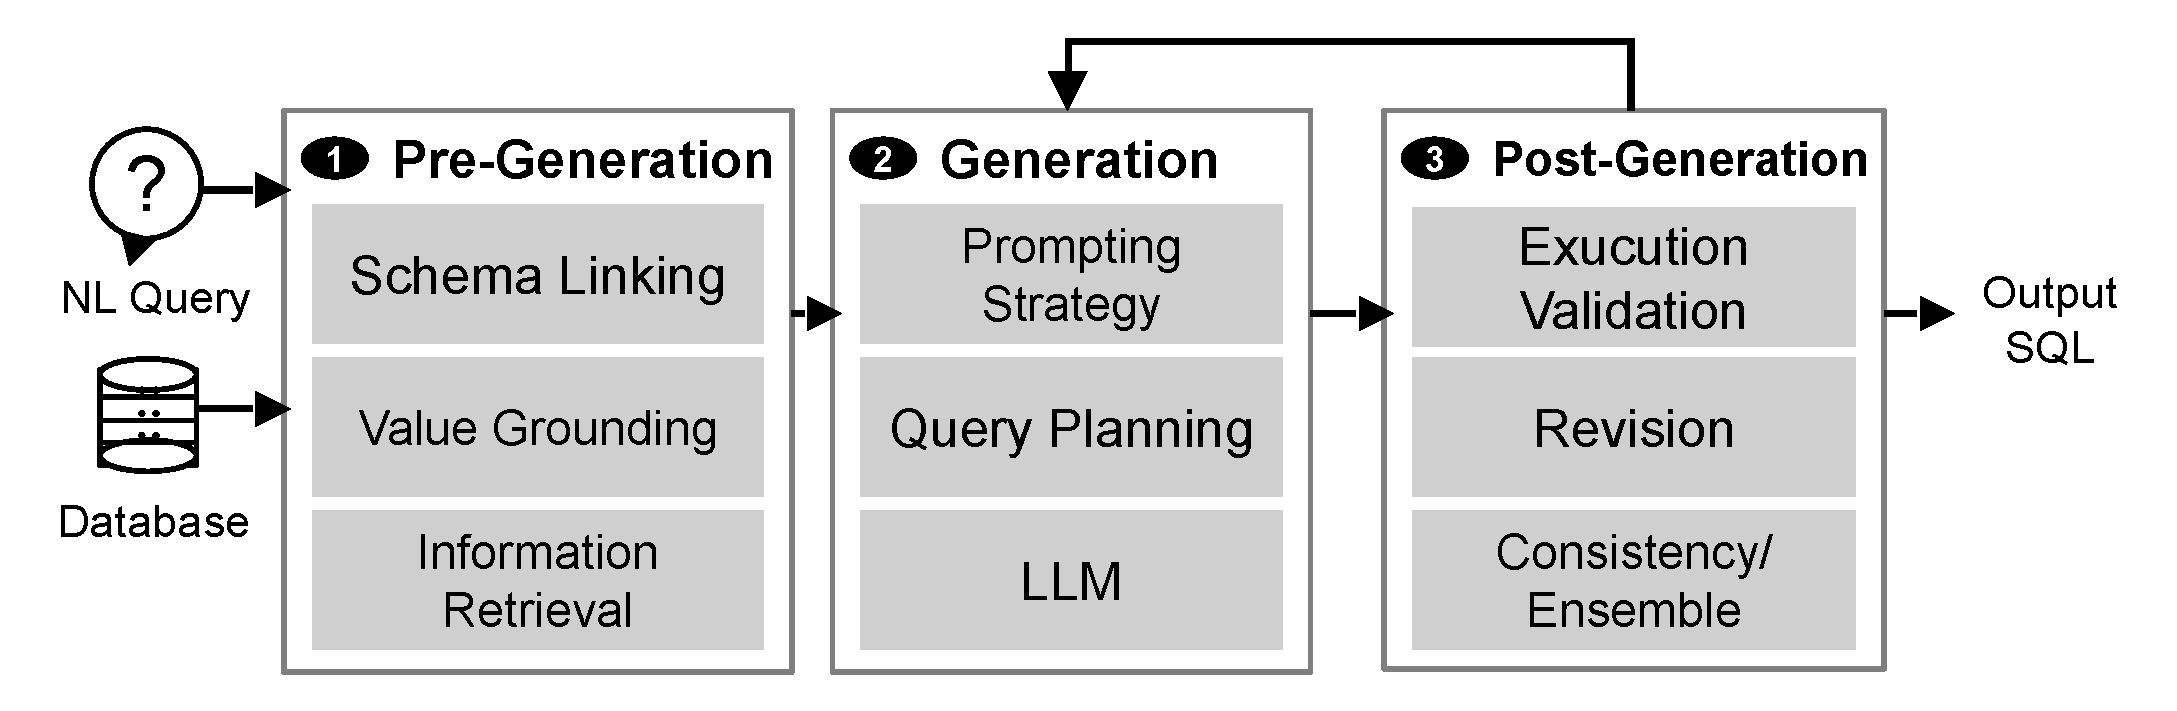
\includegraphics[width=1\linewidth]{./images/text-to-sql pipline.pdf} 
	\vspace{-5mm}
	\caption{\textbf{Overview of a typical Text-to-SQL pipeline, illustrating the Pre-Generation, Generation, and Post-Generation stages}}
	\label{fig:text-to-sql-pipeline}
	\vspace{-4mm}
\end{figure}

% 第3-5段，3个Limitations
%确实有一些工作开始做“自适应”，但多数只覆盖局部策略，而不是你这种结合环境感知、self-reflection、workflow/strategy selection 和 efficiency optimization 的 meta-cognitive controller。
%\textsc{CHESS} 会基于问题复杂度和上下文大小调整 schema pruning，但主要是 schema filtering 层面的自适应，不是全局 workflow selection。
%\textsc{QCMA-SQL} 明确做 question classification，并为不同复杂度问题调用不同 agents，比较接近“按难度选策略”。
%\textsc{OpenSearch-SQL} 提到 dynamic few-shot strategy 和 consistency alignment，更偏向 few-shot retrieval/selection 的局部自适应。
%还有一篇很新的 \textsc{SquRL} / “Beyond Static Pipelines” 直接批评 static pipeline，并通过强化学习学习动态 workflow；如果你后面 related work 要写，它可能需要重点区分。
%Although recent Text-to-SQL systems have introduced local adaptive mechanisms, such as difficulty-aware decomposition, adaptive schema pruning, dynamic demonstration retrieval, question-level agent routing, and even learned workflow policies, these adaptations are usually confined to specific stages of the pipeline.
%They provide limited support for jointly adapting the overall workflow, generation strategy, reflection behavior, and optimization effort according to the database environment, question difficulty, intermediate feedback, and execution efficiency.
% 我觉得需要讨论一下了
\textbf{L1: Limited Adaptation in Workflows and Strategy Selection.}
Many existing Text-to-SQL agents often predefine both the workflow structure and the strategy choices, where modules such as schema linking, few-shot retrieval, question decomposition, candidate generation, validation, and revision are applied in a largely fixed manner~\cite{gao2023text,pourreza2023din,wang2023mac,chaturvedi2025sqlthought,pham2026avsql}.
Although such designs improve robustness over single-shot generation, they provide limited support for adapting reasoning strategies to the current database environment, question difficulty, or intermediate feedback.
This can misallocate reasoning effort: simple queries over intuitive schemas may incur unnecessary token and latency overhead, while difficult queries may require deeper grounding, candidate comparison, or additional validation and reflection.
This mismatch is illustrated by the different effects of domain-specific hints in \textsc{BIRD}~\cite{li2023can}.
For an intuitive database such as \texttt{superhero}, where tables and columns are relatively descriptive, adding domain hints provides little additional benefit in our experiments.
In contrast, for a domain-heavy database such as \texttt{thrombosis\_prediction}, where terms such as \texttt{LDH} and gender-dependent uric-acid ranges require medical knowledge, the same hints improve accuracy from 20\% to nearly 50\%.
This contrast suggests that Text-to-SQL agents should adapt their grounding and generation strategies to the database environment, rather than applying the same strategy uniformly.

% 参考 MaCTG: Multi-Agent Collaborative Thought Graph for Automatic Programming
\textbf{L2: Post-hoc rather than Process-level Reflection.}
Feedback in many Text-to-SQL systems is mainly used after a candidate SQL has been generated, such as repairing execution errors, revising invalid queries, or selecting among completed candidates~\cite{pourreza2023din,wang2023mac,talaei2024chess,lei2024spider}.
Such feedback improves final-output validation, but provides limited support for monitoring and regulating the generation process itself.
In particular, the agent often lacks a controller that continuously tracks whether schema linking is reliable, whether candidate disagreement is increasing, whether repeated repairs are converging, or whether the current strategy should be changed.
As a result, early mistakes in schema linking, value grounding, or query planning may propagate into later steps and become cascading hallucinations.
Moreover, without global process supervision, local repair actions may fix surface-level execution errors while leaving the overall reasoning trajectory insufficiently grounded in the user question and database context.

\textbf{L3: Limited Awareness of Query Efficiency.}
Most existing Text-to-SQL systems are primarily optimized for correctness: they aim to generate SQL queries whose execution results match the ground-truth answers~\cite{li2023resdsql,li2024codes,li2023graphix,rai2023improving,scholak2021picard,wang2019rat,gao2023text,pourreza2023din}.
However, in practical database applications, a semantically correct SQL query is not necessarily efficient.
Equivalent or near-equivalent SQL formulations may lead to very different execution costs due to redundant projections, unnecessary joins, correlated subqueries, missing filter pushdown, suboptimal join orders, or functions applied to indexed columns~\cite{chaudhuri1998overview,leis2015good,wang2022wetune}.
Although database systems have long relied on rule-based, cost-based, and learned rewriting to improve query efficiency~\cite{selinger1979access,wang2022wetune,zhou2023learned,li2024llm}, current Text-to-SQL agents usually use database feedback mainly to check executability or result consistency.
They rarely treat execution plans, estimated costs, or bottleneck patterns as signals for deciding whether and how to rewrite the generated SQL.
As a result, the final query may be correct but unnecessarily expensive, especially in enterprise settings with large schemas, large tables, and long multi-step analytical workflows~\cite{lei2024spider}.


% 第六段  key insights
\textbf{Key Insights: Meta-cognitive and Environment-aware Text-to-SQL.}
Inspired by enactive cognition and meta-cognition, we view Text-to-SQL not as a static translation from question and schema to SQL, but as an adaptive interaction process between the agent and the database environment~\cite{varela1991embodied,flavell1979metacognition}.
Enactive cognition suggests that understanding is shaped through interaction with the environment, while meta-cognition emphasizes the ability to monitor and regulate one's own reasoning process.
In the context of Text-to-SQL, this means that an agent should perceive database-specific signals, act by generating and rewriting SQL, observe feedback from execution and query plans, and adjust its strategy when uncertainty, failure, or inefficiency is detected.
These perspectives lead to three design objectives.
First, to address \textbf{L1}, the agent should perform \emph{environment-aware workflow adaptation via strategy selection}: it should select lightweight or deep workflows according to the perceived database environment, question complexity, and intermediate feedback, rather than applying the same strategy uniformly.
Second, to address \textbf{L2}, the agent should support \emph{process-level self-reflection and dynamic control}: it should monitor schema-linking reliability, candidate disagreement, repair convergence, and strategy suitability during generation, so that early mistakes can be corrected before they propagate.
Third, to address \textbf{L3}, the agent should enable \emph{execution- and plan-aware SQL optimization}: it should use query plans, cost signals, semantic validation, and reusable rewrite knowledge to improve query efficiency while preserving correctness.

% 第七段 approach

% 第八段 evaluation

% 第九段 contributions


	\section{Design Objective}
\label{sec:preliminaries}

\subsection{Task Formulation}
Traditional Text-to-SQL aims to translate a NL question $x$ into an executable SQL query $q$ over a database environment $\mathcal{D}$.
Given a ground-truth query $q^*$, the standard objective is to generate a query whose execution result matches that of $q^*$:
\[
f_\theta(x, \mathcal{D}) \rightarrow q,
\quad
\text{s.t.} \quad
\text{Exec}(q, \mathcal{D}) = \text{Exec}(q^*, \mathcal{D}),
\]
where $f_\theta$ denotes a Text-to-SQL model parameterized by $\theta$, $\mathcal{D}$ denotes the database environment including schema, data, indexes, and statistics, and $\text{Exec}(q, \mathcal{D})$ denotes the result of executing $q$ on $\mathcal{D}$.

However, this formulation focuses mainly on semantic correctness and does not explicitly consider query efficiency.
In practice, multiple semantically equivalent SQL queries may produce the same result but incur substantially different execution costs due to join order, predicate placement, aggregation strategy, or index utilization.
We therefore formulate \textbf{Efficiency-Oriented Text-to-SQL}, where the goal is to generate a query that is both semantically correct and efficient.
Given a NL question $x$ and a database environment $\mathcal{D}$, the goal is to generate a SQL query $q_{\text{opt}}$ satisfying:
\[
\begin{aligned}
	q_{\mathrm{opt}}
	&= \arg\min_{q \in \mathcal{Q}_{\mathrm{corr}}(x,\mathcal{D})}
	\; \text{Cost}(q,\mathcal{D}), \\
	\mathcal{Q}_{\mathrm{corr}}(x,\mathcal{D})
	&= \{q \in \mathcal{Q}(x,\mathcal{D}) \mid \text{Exec}(q,\mathcal{D}) = \text{Exec}(q^*,\mathcal{D})\},
\end{aligned}
\]
where $\mathcal{Q}_{\mathrm{corr}}(x,\mathcal{D})$ denotes the subset of candidates that are semantically correct with respect to $q^*$.
$\text{Cost}(q, \mathcal{S})$ represents the estimated or actual execution cost of query $q$ on $\mathcal{S}$.
Intuitively, the model should not only ensure that $q_{\text{opt}}$ yields correct results but also that it achieves minimal execution time or resource consumption under the same semantic constraints. 


%	\section{EESQLBench}
\label{sec:EESQLBench}

In this section, we introduce the construction of \benchmark , the first benchmark for evaluating Efficiency-Oriented Text-to-SQL tasks.
Figure \ref{fig:overview} illustrates the entire process involved in building our benchmark.
Starting from real-world databases, we enhance database schemas and data instances to expose performance-sensitive behaviors, and generate   complex SQL queries that admit substantial optimization opportunities.
For each generated query, we further curate a semantically equivalent but efficiency-optimized canonical SQL via automated rewriting and expert refinement, and align it with a natural language (NL) question.
More details will be introduced in the following subsections.

\subsection{Benchmark Construction}
% Implementation

\begin{figure}[t]
	\centering
	\includegraphics[width=0.9\linewidth]{./images/Overview.pdf} 
	\vspace{-5mm}
	\caption{\textbf{Overview of \benchmark\ Construction Pipeline}}
	\label{fig:overview}
	\vspace{-5mm}
\end{figure}

\subsubsection{Database Preparation.}
We prepare the databases of \benchmark\ by building upon real-world relational databases collected from the \textsc{BIRD}~\cite{li2023can} benchmark.
We choose \textsc{BIRD}~\cite{li2023can} because it covers cross-domain scenarios spanning diverse application areas, including e-commerce, finance, and healthcare, and provides large-scale tables derived from real-world data with rich relational structures and realistic data distributions.
Based on these databases, we enhance the original schemas to better support efficiency-oriented evaluation.
% 修复外键
In particular, we explicitly repair missing or implicit foreign-key relationships, which enables multiple alternative join paths among related tables and allows semantically equivalent SQL queries to be expressed in structurally different forms.
% 随机添加索引
We further apply mixed indexing strategies by randomly indexing a subset of foreign-key and attribute columns, so that different join orders and access paths can lead to distinct execution plans. 
% 插入数值和噪声数据，数据分布
At the instance level, we enlarge the databases by systematically inserting additional rows into existing tables while strictly preserving the original schemas, data types, and foreign-key constraints.
For each table, new tuples are generated by sampling valid key values from referenced tables and duplicating existing records with controlled variations on non-key attributes.
We explicitly control value frequencies for selected predicate-relevant attributes by making some values significantly more frequent than others, thereby introducing skewed data distributions that amplify efficiency differences among semantically equivalent queries.


\subsubsection{Complexity-Aware Query Generation.}
After preparing databases, we synthesize SQL queries that are both structurally complex and optimization-sensitive.
We adopt a reverse construction strategy: instead of starting from NL and hoping a generator produces sufficiently challenging SQL, we first generate complex SQL candidates and then align them with NL questions.
%Our design is inspired by DBMS fuzzing, which is effective at exploring a wide spectrum of query structures (e.g., deep nesting, multi-join chains, and aggregation patterns) that can expose optimizer behaviors.
%However, directly using off-the-shelf fuzzers often yields many ill-typed, semantically invalid, or practically meaningless queries, while directly prompting an LLM tends to produce overly ``clean'' and repetitive SQL due to pretraining biases.
%This means LLM-generated queries often exhibit limited structural diversity, favoring simple join patterns and shallow nesting that provide few opportunities for efficiency-sensitive analysis.
Our design is inspired by DBMS fuzzing, which can explore a wide spectrum of query structures (e.g., deep nesting, multi-join chains, and aggregation patterns) that are useful for stress-testing optimizer behavior.
However, off-the-shelf fuzzers are not directly applicable: they often produce ill-typed, semantically invalid, or practically meaningless queries.
On the other hand, prompting an LLM can improve semantic plausibility and executability, but the generated SQL is often overly ``clean'' and repetitive due to pretraining biases, favoring simple join patterns and shallow nesting.
As a result, neither approach alone can simultaneously provide high structural diversity and semantic validity.
To balance these two objectives, we introduce a \emph{SQL Sketch} mechanism that decouples \emph{query structure} from \emph{schema-specific semantics}.
As illustrated in Figure~\ref{fig:sql template}, query generation proceeds in two stages: (i) grammar-based SQL sketch generation, which generates the high-level relational structure of a query, and (ii) LLM-based instantiation, which binds schema-dependent elements under explicit constraints.

\begin{figure}[t]
	\centering
	\includegraphics[width=1\linewidth]{./images/SQL template.pdf} 
	\vspace{-8mm}
	\caption{\textbf{Two-Stage Query Generation via Grammar-Based SQL Sketching and LLM-Based Instantiation}}
	\label{fig:sql template}
	\vspace{-7mm}
\end{figure}

\textbf{(1) Grammar-Based SQL Sketch Generation.}
We firstly generate SQL sketches by sampling from a context-free grammar that specifies optimization-sensitive query structures.
We implement this grammar as shown in Figure \ref{fig:sql template} and use \textsc{go-randgen}~\cite{go-randgen} as a grammar-based generator to derive grammar-valid sketches, covering patterns such as multi-table joins, nested subqueries, common table expressions (CTEs), and aggregations with \texttt{HAVING} clauses.
By construction, each sketch fixes the high-level composition and nesting of relational operators, while abstracting away schema-specific details.
Concretely, schema-dependent elements—including table names, column references, join predicates, and literal constants—are replaced with typed placeholders (denoted by identifiers prefixed with an underscore, e.g., \texttt{\_table}, \texttt{\_cte\_table}, \texttt{\_column}, \texttt{\_agg\_func}, \texttt{\_const}).
This sketch-based design ensures structural correctness and diversity at the query level, while deferring schema binding and semantic instantiation to a later stage.

\textbf{(2) LLM-based Query Instantiation.}
Given a target database, we prompt an LLM to instantiate each sketch by filling placeholders with concrete tables, columns, predicates, and values.
To improve semantic plausibility and controllability, the instantiation prompt includes the following components:
\begin{itemize}[leftmargin=10pt]
	\item \textbf{Task Instruction:} Instructs the LLM to fill the provided SQL sketch into an executable query that corresponds to a meaningful analysis intent, rather than producing arbitrary or trivial SQL.
	\item \textbf{Database Schema:} Provides the full \texttt{CREATE TABLE} statements (table names, columns, types, primary keys, and foreign keys) so that the LLM can select type-consistent columns and produce join conditions aligned with the schema constraints.
	\item \textbf{Database Values:} Samples representative values for a few columns (e.g., categorical values, typical timestamps, common IDs) to ground predicate generation, reducing ill-formed conditions (e.g., comparing strings to numeric columns) and improving contextual relevance.
%	\item \textbf{Column Selection Constraint:} Specifies the target number of output columns (e.g., sampled from a small-biased distribution) so that the generated query returns a concise result schema, consistent with common user-facing analytical questions that focus on a few key attributes.
	\item \textbf{Few-shot Examples:} Provides a small number of example queries following the same formatting and style, helping the LLM adhere to the desired SQL conventions (e.g., aliasing, indentation, and aggregation style).
\end{itemize}
The LLM is explicitly instructed to satisfy typing constraints and foreign-key connectivity when instantiating placeholders, producing executable SQL candidates.

Finally, we validate each instantiated query through execution.
Queries that fail to parse, violate schema constraints, or produce empty results are discarded.
%Only queries that execute successfully and exhibit non-trivial intermediate data processing are retained.
This process results in a large pool of complex and semantically meaningful SQL queries that admit substantial optimization opportunities, which are used in subsequent canonicalization and question alignment.

\subsubsection{Efficient Query Construction.}
For each synthesized SQL query, our goal is to construct a semantically equivalent but execution-efficient canonical query that represents expert-level optimization.
To this end, we adopt a two-stage optimization pipeline that combines automated query rewriting with expert refinement, and explicitly annotate the applied optimization types.
As a first step, we apply an automated query rewriting procedure to identify candidate efficiency improvements.
Specifically, we leverage \textsc{WeTune}~\cite{wang2022wetune}, a rule-based query rewriting framework, to generate semantically equivalent query variants through systematic application of rewriting rules.
For each original query, we evaluate the rewritten variants and retain those that exhibit reduced execution cost.
Building upon the automatically rewritten candidates, database experts further refine the queries to produce a final optimized canonical SQL.
% 专家的选择
In this project, we engage three full-time Text-to-SQL experts, all of whom are Ph.D. students with formal training in hands-on experience in SQL optimization and query tuning. 
The entire expert refinement process for all queries takes approximately 80 person-hours in total.
During this stage, experts manually inspect query structures and execution plans, and apply domain knowledge to introduce deeper optimizations that are difficult to fully capture by rule-based systems.
In addition, we explicitly annotate the primary optimization types applied to each query pair.
Each query pair is labeled with one or more optimization categories indicating where efficiency gains are achieved, such as \emph{join reordering}, \emph{predicate pushdown}, \emph{subquery elimination}, and \emph{aggregation rewriting}.
For example, if an optimized query achieves lower execution cost by pushing a filtering predicate from an outer query into an inner subquery before aggregation, it is annotated with \emph{predicate pushdown}.
These annotations enable fine-grained analysis of Text-to-SQL systems’ optimization capabilities.


\subsubsection{Natural Language Question Alignment.}
After constructing pairs of semantically equivalent original and optimized SQL queries, we align them with NL questions that faithfully capture the underlying analytical intent.
The key design principle of this stage is to ensure fairness: each NL question should reflect the high-level user intent of the query, without encoding any SQL-specific structures or optimization decisions.
To achieve this, we generate NL questions based on the shared semantics of each original–optimized query pair, rather than directly mirroring either concrete SQL formulation.
Specifically, we adopt a back-translation strategy in which an LLM is prompted to translate a given SQL query into a concise and natural NL question.
Importantly, the prompt provides both the original SQL and the optimized canonical SQL as semantic references, and explicitly instructs the model to generate a question that is simultaneously satisfied by both queries.
Concretely, the prompt is constructed with the following components:
\begin{itemize}[leftmargin=10pt]
	\item \textbf{Task Instruction.} 
	The model is instructed to generate a NL question that describes the analytical goal of the queries—i.e., what information is requested—rather than how the result is computed.
	
	\item \textbf{Dual Semantic References.} 
	Both the original SQL query and its optimized canonical counterpart are provided as semantic references.
	The model is instructed to infer the common analytical intent underlying the two queries and generate a single NL question that is valid for both, treating the SQLs as black-box specifications of the result.
	
	\item \textbf{Implementation Abstraction Constraint.} 
	The prompt explicitly prohibits mentioning SQL-specific constructs, such as joins, subqueries, aggregation operators, execution order, or optimization strategies, and requires the question to be phrased in natural, user-centric terms.
	
	\item \textbf{Semantic Equivalence Constraint.} 
	The generated question must remain answerable by any semantically equivalent SQL formulation, ensuring neutrality with respect to different query structures and execution strategies.
\end{itemize}
Following generation, all NL questions undergo a human verification and refinement step.
Three experts check each question for semantic alignment with both SQL variants, clarity, and naturalness, and revise ambiguous or overly verbose descriptions when necessary.
As a result, each NL question in \benchmark\ represents a realistic, user-facing query intent, and that can be correctly answered by multiple semantically equivalent SQL queries.
This alignment strategy enables \benchmark\ to simultaneously evaluate (i) semantic correctness, by checking whether a model-generated SQL answers the NL question correctly, and (ii) efficiency awareness, by comparing the execution efficiency of the generated SQL against the expert-optimized canonical query.

\subsubsection{Quality Control and Annotations.}
\label{subsubsec:quality control}
In the final stage, we conduct quality control for each Text-to-SQL task to ensure the correctness, consistency, and reliability of the benchmark.
This stage consists of semantic consistency verification and task difficulty annotation.

\textbf{(1) Semantic consistency verification.}
We first verify the semantic consistency of each task across both SQL queries and the corresponding NL question.
Specifically, we check that the original SQL query and the optimized SQL query are semantically equivalent by executing them under the same database configuration and comparing their result sets.
Meanwhile, we require the optimized query to consistently achieve lower execution cost, ensuring the presence of a genuine and stable efficiency gap.
We further verify that the NL question can be correctly answered by both SQL queries, confirming that it accurately captures their shared analytical intent.

\textbf{(2) Task difficulty annotation.}
After passing semantic consistency verification, we annotate the difficulty of each Text-to-SQL instance using a rule-based human scoring scheme along three complementary dimensions:
\begin{itemize}[leftmargin=10pt]
	\item \textbf{Schema Complexity:} the number of involved tables, join relationships, and foreign-key dependencies;
	\item \textbf{Question Understanding:} the presence of multiple conditions, implicit constraints, or required reasoning in the NL question;
	\item \textbf{SQL Complexity:} the structural and operator-level complexity of the query, such as subqueries, aggregations, \texttt{HAVING} clauses, and CTEs.
	%	SQL 复杂性是根据 Optimized 的判断的
\end{itemize}
Each dimension is graded according to predefined criteria specified in the annotation guidelines~\cite{eesqlbench_guidelines}, and the final difficulty label (e.g., Simple, Medium, or Hard) is determined by aggregating the scores across all dimensions.

All verification and annotation procedures are conducted by three domain experts.
Two experts independently evaluate each instance following a unified guideline, and disagreements are resolved by a third expert acting as an adjudicator.
We measure inter-annotator agreement using Cohen’s kappa coefficient, obtaining an overall kappa score of 0.92, which indicates high annotation consistency and reliable quality.
As a result, each task in \benchmark\ is accompanied by structured annotations, including the database context, paired original and optimized SQL queries, a shared NL question, explicit optimization-type labels, and a difficulty level.
These annotations provide a reliable foundation for analyzing both semantic correctness and optimization awareness of Text-to-SQL systems.

\subsection{Statistics}

\begin{wrapfigure}{r}{0.45\textwidth}
	\vspace{-14mm}
	\centering
	\includegraphics[width=0.45\textwidth]{./images/DB Complexity.pdf}
	\vspace{-5mm}
	\caption{\textbf{Distributions of Database Size in \benchmark\ (Log Scale)}}
	\label{fig:statistics}
	\vspace{-4mm}
\end{wrapfigure}
We present a statistical analysis of \benchmark\ and compare it with representative Text-to-SQL benchmarks in Table~\ref{tab:text2sql_stats}.
\benchmark\ is constructed on MySQL as the execution backend.
Overall, \benchmark\ contains \tasknumber\ Text-to-SQL tasks over 69 real-world databases.
All tasks are manually curated and paired with expert-optimized canonical SQL queries, enabling direct efficiency comparison between model-generated SQL and expert-level solutions.
Following a unified guideline (Section~\ref{subsubsec:quality control}), we further label each task with a difficulty level, resulting in 55 Simple, 85 Medium, and 73 Hard tasks.

%Figure~\ref{fig:statistics} shows the distribution of database sizes in \benchmark\ (log scale).
Figure~\ref{fig:statistics} shows the distribution of database sizes in \benchmark\ on a log scale; for completeness, we provide a detailed breakdown of record counts in our online documentation~\cite{eesqlbench_database_size}.
\benchmark\ covers databases with highly heterogeneous instance scales, spanning from 148kB to 4.4 GB.
In addition, \benchmark\ is explicitly designed to be efficiency-aware at three levels.
At the \emph{schema level}, each database contains 7.75 tables on average (and up to 65), with repaired foreign-key relationships that enable multiple semantically equivalent join paths.
At the \emph{instance level}, each database contains 3,432,599 records on average, and we further introduce controlled table-scale imbalance and value-frequency skew to amplify cost gaps among semantically equivalent queries.
At the \emph{query level}, each task involves 3.55 tables on average (up to 11) and 2.88 subqueries on average (up to 8), resulting in a substantial portion of multi-join and nested queries that admit non-trivial optimization opportunities.



\section{Efficiency-Oriented Evaluation Metrics}
\label{sec:metrics}
%1、EX
%2、在EX通过的基础上统计 Execution Time 、Actual Rows？
%3、计算与人工解的比值？

Evaluating Efficiency-Oriented Text-to-SQL requires metrics that not only assess semantic correctness but also reliably quantify query execution efficiency. 
While execution latency is a natural indicator of efficiency, it is highly sensitive to external factors, making it unstable and difficult to reproduce. 
Therefore, we adopt query-plan-based cost metrics, which provide a more stable proxy for intrinsic query efficiency.

\paragraph{Semantic Correctness.}
We first evaluate whether a generated query $\hat{q}$ is semantically equivalent to the canonical query $q^*$.
Following prior works~\cite{yu2018spider,li2023can}, semantic equivalence is determined by comparing execution results:
\[
\mathbf{1}(q^*, \hat{q}) =
\begin{cases}
	1, & \text{if } \text{Exec}(\hat{q}, \mathcal{S}) = \text{Exec}(q^*, \mathcal{S}), \\
	0, & \text{otherwise}.
\end{cases}
\]
Efficiency-related metrics are computed only on semantically correct queries (i.e., those with $\mathbf{1}(q^*, \hat{q}) = 1$), ensuring that efficiency evaluation is not confounded by incorrect query semantics.

\paragraph{\textbf{Cost Reachability (CR)}}
To measure a model-generated query's proximity to expert-level efficiency,
we introduce \emph{Cost Reachability (CR)}.
For each semantically correct query pair $(q^*, \hat{q})$, we define:
\[
CR_n = \frac{\text{Cost}(q^*, \mathcal{S})}{\text{Cost}(\hat{q}, \mathcal{S})},
\]
where $\text{Cost}(q, \mathcal{S})$ denotes the execution cost of query $q$ on schema $\mathcal{S}$, 
obtained from the query execution plan.
A larger $CR_n$ indicates that the generated query $\hat{q}$ is more efficient relative to the canonical solution $q^*$, 
while $CR_n < 1$ implies inferior efficiency.

To mitigate the influence of extreme outliers, we follow prior cost-based evaluation practices~\cite{li2023can} and apply a square-root transformation to obtain a stabilized score:
\[
R_n = \sqrt{CR_n}.
\]
The overall Cost Reachability is then computed as:
\[
CR_{\text{avg}} =
\frac{1}{\sum_{n=1}^{N} \mathbf{1}(q^*_n, \hat{q}_n)}
\sum_{n=1}^{N} \mathbf{1}(q^*_n, \hat{q}_n) \cdot R_n,
\]
where $N$ is the total number of evaluation instances. For brevity, we use CR to refer to the aggregated score $CR_{\text{avg}}$ in the remainder of the paper.

\paragraph{\textbf{Acceptable Reachability at $k$ (AR@$k$).}}
While $CR_{\text{avg}}$ characterizes the efficiency gap \emph{conditioned on semantic correctness}, it does not reflect how often a model produces queries that are both correct and practically efficient.
To capture this end-to-end utility, we define \emph{Acceptable Reachability at $k$} (AR@$k$) as:
\[
AR@k =
\frac{1}{N}
\sum_{n=1}^{N} \mathbf{1}(q^*_n, \hat{q}_n) \cdot \mathbf{1}(CR_n \ge k),
\]
where $k \in (0,1]$ is a user-defined threshold.
Intuitively, AR@$k$ measures the fraction of all test instances for which the generated SQL is semantically correct and its execution cost does not exceed $1/k$ times that of the canonical solution.
For example, $k=0.5$ corresponds to accepting queries that are at most twice as expensive as the expert-optimized SQL, while $k=1.0$ only counts queries whose execution cost is no higher than the canonical solution (i.e., at least as efficient as the expert-optimized SQL).

Together, CR and AR@$k$ provide complementary perspectives on efficiency:
CR measures \emph{how close} a model can get to expert-level efficiency on average (given correctness),
while AR@$k$ measures \emph{how often} it produces SQL that is both correct and meets a practical efficiency threshold.


	\section{OptSQL}
\label{sec:OptSQL}

\subsection{Overview}
Figure~\ref{fig:overview} shows the overall architecture of \toolname.
Given a NL question and a database environment, \toolname\ aims to generate a SQL query that is both semantically correct and execution-efficient.
Instead of treating Text-to-SQL as a fixed pipeline, \toolname\ formulates it as a feedback-driven process coordinated by a Meta-Cognitive Controller.
%
The Meta-Cognitive Controller supervises the entire workflow.
It perceives the database environment, estimates the difficulty of the input question, selects suitable actions, and monitors intermediate feedback throughout both generation and optimization.
Under its control, \toolname\ first constructs an initial SQL query in the Generation Phase, where an evidence-guided schema filter identifies relevant tables, columns, values, and join paths, and an initial SQL builder produces executable candidate queries.
If the controller detects that the query requires further efficiency improvement, it activates the Optimization Loop.
This loop consists of an Explain Analyzer Agent, a SQL Rewriter Agent, and a Validator Agent, which together analyze execution plans, rewrite inefficient SQL patterns, and verify semantic consistency and cost reduction.
%
\toolname\ is further supported by a Memory Engine and a Tool Infrastructure.
The Memory Engine maintains both task-level working memory and reusable optimization knowledge, including expert rules, historical rewrite cases, and observed optimization patterns.
The Tool Infrastructure provides database grounding, SQL execution and analysis, cost evaluation, semantic consistency checking, and RAG-based retrieval.
Through these components, \toolname\ continuously observes feedback from the database environment, reflects on its intermediate decisions, and updates its optimization experience.

\begin{figure*}[t]
	\centering
	%	\vspace{-3mm}
	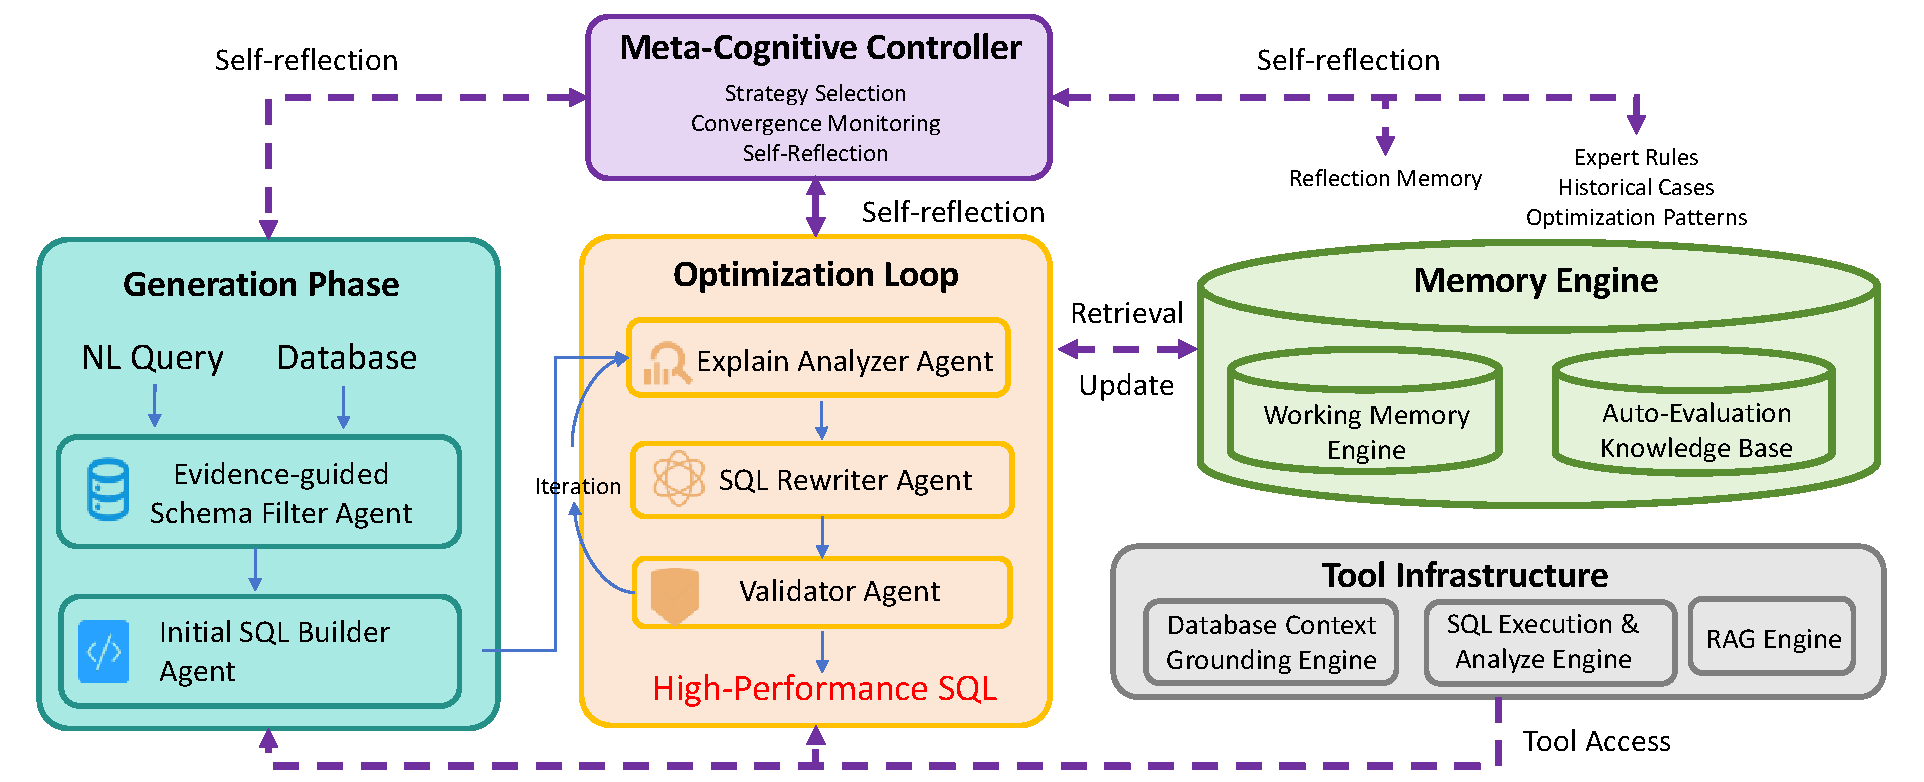
\includegraphics[width=1\linewidth]{./images/overview.pdf} 
	\vspace{-5mm}
	\caption{\textbf{Overview of \toolname}}
	\label{fig:overview}
	\vspace{-4mm}
\end{figure*}

The remainder of this section describes each component of \toolname.
We first present the Generation Phase for constructing an initial SQL query (Section~\ref{subsec: Generation Phase}), followed by the Optimization Loop for execution-aware rewriting (Section~\ref{subsec: Optimization Loop}).
We then introduce the Meta-Cognitive Controller that orchestrates these processes through strategy selection, monitoring, and self-reflection (Section~\ref{subsec: Meta-Cognitive Controller}).
Finally, we describe the Memory Engine and Tool Infrastructure that support retrieval, experience accumulation, and database feedback (Section~\ref{subsec: Memory Engine and Tool Infrastructure}).

\subsection{Generation Phase}
\label{subsec: Generation Phase}
The Generation Phase aims to construct a set of executable and semantically plausible initial SQL candidates based on the question and database environment.
It focuses on two core capabilities: evidence construction and multi-strategy SQL generation, without global control or optimization decisions.

\textbf{Evidence-guided Schema Filter Agent.}
This agent is responsible for grounding the input question into a compact, relevant, and executable schema context for downstream SQL generation.
This agent is responsible for grounding the input question into a compact, relevant, and executable schema context for downstream SQL generation.
It combines robust schema linking with value-level grounding, aiming to identify not only the tables and columns mentioned or implied by the question, but also the concrete database values and conditions needed to express the user intent.
To improve schema robustness, the agent supports multiple complementary schema linking strategies:

\begin{itemize}[leftmargin=10pt]
	\item \textit{Direct schema linking} maps the natural language question to relevant tables and columns by reasoning over question semantics and schema descriptions.
	This strategy is effective when the question contains explicit lexical or semantic cues.
	
	\item \textit{Reverse schema linking} hypothesizes a tentative SQL structure and then extracts the tables and columns implied by this structure~\cite{li2026deepeye}.
	This recovers latent schema dependencies, such as join tables, grouping columns, or aggregation-related attributes, that may be missed by direct matching.
	
	\item \textit{Value-grounded schema linking} identifies relevant schema elements through actual database contents.
	Instead of relying only on table or column names, the agent checks whether values in a column match or semantically correspond to phrases in the question, which is especially useful when schema names are ambiguous or weakly informative.
\end{itemize}

Beyond schema linking, the agent further performs active value grounding to translate natural language expressions into concrete database predicates.
It supports several value grounding capabilities:

\begin{itemize}[leftmargin=10pt]
	\item \textit{Exact value verification} checks whether a phrase in the question directly appears in candidate columns.
	This is useful for grounding categorical conditions such as names, locations, statuses, or labels.
	
	\item \textit{Semantic value matching} retrieves column values that are semantically close to question phrases, allowing the agent to handle paraphrases, abbreviations, and domain-specific expressions.
	
	\item \textit{Distinct-value inspection} examines representative or unique values of a column to infer how natural language concepts are encoded in the database, such as whether a Boolean concept is represented by \texttt{0}/\texttt{1}, \texttt{Y}/\texttt{N}, or textual labels.
	
	\item \textit{Data sampling and distribution checking} inspects example rows or value distributions to understand column semantics and avoid grounding predicates on irrelevant or sparsely populated columns.
	
	\item \textit{Null and type analysis} checks whether candidate columns contain nulls or unexpected value formats, helping the agent avoid unreliable predicates and distinguish categorical, numerical, date, and Boolean constraints.
	
	\item \textit{Composite predicate grounding} combines multiple grounded values or columns when a natural language phrase corresponds to a compound condition, such as a grade span, date range, or multi-attribute status.
\end{itemize}

For example, a phrase such as ``kindergarten to 8th grade'' may be grounded as \texttt{Low\_Grade = 'K'} and \texttt{High\_Grade = '8'}, while ``magnet program'' may correspond to a binary or categorical value after inspecting the value distribution of a related column.
These grounded facts are passed to the SQL generator as explicit evidence, reducing the risk of hallucinated predicates or incorrect value choices.
Finally, the agent further completes the relational context required for SQL construction.
The selected schema elements may be semantically relevant but structurally disconnected; for example, two relevant tables may require intermediate tables or primary--foreign key columns to form a valid join path.
Therefore, the agent supplements necessary join keys and bridge tables according to the database relationships, so that the resulting schema context can support executable SQL generation.
The output of this agent is an evidence-enriched schema context that integrates schema relevance, verified value grounding, ambiguous-case evidence, and join-path information for downstream SQL generation.

\textbf{Initial SQL Builder Agent.}
Initial SQL Builder Agent is responsible for producing executable and semantically plausible initial SQL candidates.
It provides a set of complementary SQL construction capabilities, rather than a fixed generation pipeline.
Depending on the task complexity, schema ambiguity, and control signals from the Meta-Cognitive Controller, the agent may invoke one or more generation strategies to balance robustness and efficiency.
The agent supports the following SQL generation strategies:

\begin{itemize}[leftmargin=10pt]
	\item \textit{Skeleton-based generation} follows a top-down construction process.
	It first analyzes the required SQL components, such as selection, filtering, joining, grouping and ordering, then sketches a SQL skeleton, and finally fills in concrete tables, columns, predicates, and functions.
	This strategy is useful for queries that require clear structural planning.
	
	\item \textit{ICL-based generation} leverages retrieved demonstrations to guide SQL construction.
	By retrieving structurally similar examples, the agent can reuse successful query patterns and adapt them to the current grounded schema.
	This strategy is especially helpful when the question resembles previously observed SQL structures.
	
	\item \textit{Decomposition-based generation} breaks a complex question into simpler sub-questions and generates SQL fragments for each sub-task before composing them into a complete query.
	This strategy is designed for complex analytical questions involving nested reasoning, multiple conditions, or multi-step aggregation.
\end{itemize}

After candidate generation, the agent can apply a lightweight repair loop to improve executability.
It checks basic syntactic and execution errors, and revises invalid candidates using the original question, grounded schema evidence, and database error messages.
This repair process removes obvious generation failures before candidate selection, while leaving global strategy switching and deeper optimization to the Meta-Cognitive Controller.
When multiple candidates are available, the agent further supports \textit{execution-based selection}.
Candidates are grouped according to their execution results, and each group is treated as a behavioral cluster.
If one cluster forms a dominant majority, the agent selects a representative query from that cluster as the initial SQL.
Otherwise, representative candidates from the top clusters are compared through pairwise semantic judgment, and each candidate is ranked by a confidence-aware score.
%\[
%score(q) = conf(q) \times winRate(q).
%\]
The candidate with the highest score is selected as the output of the Initial SQL Builder Agent.


\subsection{Optimization Loop}
\label{subsec: Optimization Loop}

The Optimization Loop aims to improve the execution efficiency of an initial SQL query while preserving its semantics.
It is activated when the Meta-Cognitive Controller determines that the generated SQL may benefit from further optimization, such as when the query involves large tables, complex joins, or inefficient query plans.
Instead of treating SQL generation as the final step, this loop refines the initial query through execution-aware analysis, rewriting, and validation.

%\textbf{Explain Analyzer Agent.}
%This agent is responsible for diagnosing potential inefficiencies in the current SQL query.
%Given an initial SQL query, it inspects both the query structure and database feedback, including query plans, estimated costs, and observable bottleneck patterns.
%Based on this analysis, it produces optimization suggestions for the SQL Rewriter Agent.
%As shown in Table~\ref{tab:explain-analyzer}, the agent maintains a set of optimization patterns.
%Each pattern describes a possible inefficiency, a corresponding rewrite direction, and the safety condition under which the rewrite should be considered.
%These suggestions are not directly applied as deterministic rules.
%Instead, they serve as evidence for the SQL Rewriter Agent, which decides how to rewrite the query under semantic-preservation constraints.
%
%\begin{table*}[t]
%	\centering
%	\caption{\textbf{Optimization patterns used by the Explain Analyzer Agent.}}
%	\label{tab:explain-analyzer}
%	\small
%	\begin{tabular}{p{0.21\linewidth}p{0.34\linewidth}p{0.35\linewidth}}
%		\toprule
%		Pattern & Rewrite Direction & Safety Condition \\
%		\midrule
%		Redundant projection
%		& Replace \texttt{SELECT *} with necessary projected columns.
%		& Applied when required output columns can be inferred from the question or generated SQL. \\
%		
%		Scalar \texttt{MAX}/\texttt{MIN} subquery
%		& Rewrite to \texttt{ORDER BY ... LIMIT 1}.
%		& Applied only when tie behavior and aggregation semantics are preserved. \\
%		
%		Correlated subquery
%		& Rewrite to \texttt{JOIN} or \texttt{CTE}.
%		& Applied when an equivalent rewrite pattern is retrieved or can be validated. \\
%		
%		Missing filter pushdown
%		& Move selective predicates closer to base tables.
%		& Applied when predicate movement does not change join or aggregation semantics. \\
%		
%		Late aggregation
%		& Pre-aggregate before join.
%		& Applied when grouping keys and aggregation semantics remain equivalent. \\
%		
%		Inefficient \texttt{OR} predicate
%		& Rewrite to \texttt{UNION} or \texttt{UNION ALL}.
%		& Applied when duplicate semantics are correctly handled. \\
%		
%		Redundant join path
%		& Simplify unnecessary joins or bridge tables.
%		& Applied only when projected columns and filtering semantics are unaffected. \\
%		
%		Function on indexed column
%		& Rewrite to an equivalent range or comparison predicate.
%		& Applied when the transformation preserves value semantics. \\
%		
%		Inefficient ordering
%		& Align \texttt{ORDER BY} / \texttt{LIMIT} with available ordering or indexes.
%		& Applied when ordering semantics are unchanged. \\
%		\bottomrule
%	\end{tabular}
%\end{table*}
%
%\textbf{SQL Rewriter Agent.}
%This agent transforms the current SQL query into a potentially more efficient variant.
%Its input includes the original SQL, optimization suggestions from the Explain Analyzer Agent, and optionally retrieved rewrite cases or expert rules from the Memory Engine.
%The rewriter is required to preserve the original query semantics while applying only the optimization actions supported by the available evidence.
%The rewriting process focuses on producing semantically equivalent SQL variants with lower estimated or actual execution cost.
%For example, it may remove unnecessary projections, push selective predicates closer to base tables, rewrite inefficient subqueries, avoid functions on indexed columns when an equivalent range predicate is available, or restructure joins and aggregations under explicit safety constraints.
%The output of this agent is a rewritten SQL query together with a brief explanation of the applied optimization rationale.
%
%\textbf{Validator Agent.}
%This agent verifies whether the rewritten SQL is both correct and beneficial.
%It performs two checks.
%First, it checks semantic consistency between the original SQL and the rewritten SQL, ensuring that the rewrite does not change the intended result.
%Second, it evaluates whether the rewritten SQL reduces execution cost, using estimated optimizer cost, execution latency, or other available database feedback.
%If the rewritten query violates semantic consistency, the result is rejected and returned for further reflection.
%If the rewritten query preserves semantics but fails to improve cost, the loop may either retry with a different rewriting strategy or terminate when no meaningful improvement is observed.
%Only when both semantic preservation and cost reduction are satisfied is the rewritten query accepted as the optimized output.
%
%Overall, the Optimization Loop provides an execution-aware refinement mechanism for \textsc{OptSQL}.
%The Explain Analyzer Agent identifies optimization opportunities, the SQL Rewriter Agent applies evidence-guided rewrites, and the Validator Agent ensures that the rewrite is both semantically safe and performance-improving.
%Through this loop, \textsc{OptSQL} can transform an initially correct SQL query into a higher-performance query under the supervision of the Meta-Cognitive Controller.

\subsection{Meta-Cognitive Controller}
\label{subsec: Meta-Cognitive Controller}

\subsection{Memory Engine and Tool Infrastructure}
\label{subsec: Memory Engine and Tool Infrastructure}









	\section{Experiment}
\label{sec:evaluation}

% EX VES CR AR@1 AR@0.8
% Baselines:
% -  开源基础模型 + 闭源基础模型： GPT-5.4、Deepseek、Qwen-7B、XiYanSQL-7B、Llama-8B (选3-4个模型)
% -  Text-to-SQL Agentic / Approach : 
		%Multi-Agent Approach： Agentar-Scale-SQL、MAC-SQL、CHESS
%		%Single-Agent Appraoch:  DIN-SQL、DAIL-SQL
% Benchmark: BIRD and EESQLBench

% RQ1： Overall Performance  表格可以参考 LEAF-SQL: Level-wise Exploration with Adaptive Fine-graining for Text-to-SQL Skeleton Prediction、SchemaRAG
% RQ2： Ablation Study
% RQ3:  Case Study


%- BaseLines
%1. （2种）基于 Prompt 的方法：DIN-SQL，DAIL-SQL
%2. （3种）基于 Agent 的方法：
%- MAC-SQL，DeepEye
%- CHESS（需要再看一下结果）
%3. （2种）基于微调模型的方法（基于原始 BIRD pipeline）：XiYan-SQL（QwenCoder-32B-2504） + OmniSQL(32B)
%
%- LLMs
%- Qwen3-Coder-30B-A3B-Instruct
%- CodeLlama-34b-Instruct-hf
%- DeepSeek-v4-pro
%- GPT-5.4


% Performance Evaluation  (Token 消耗)
% Ablation Study
% Error Analysis

% 统计显著性检验
% 重复运行5次?


% 效率评估： 在一个model上面做就好了

%Full OptSQL
%w/o Dynamic Controller  把 Meta-Cognitive Controller 替换成固定 workflow
%w/o Process-level Reflection  只保留最终 validation/repair，不允许中间切换策略、补 evidence、重试 rewrite
%w/o Optimization Loop 生成 initial SQL 后直接输出
%w/o AEKB 不使用历史 rewrite cases，只用当前 query plan 和静态 rules



\subsection{Experimental Setup}
\textbf{Datasets.}
We evaluate \toolname\ on two complementary benchmarks: \textbf{\textsc{BIRD}}~\cite{li2023can} and \textbf{\textsc{EESQLBench}}~\cite{lin2026cracking}.
\textsc{BIRD} is a widely used cross-domain Text-to-SQL benchmark, containing more than 12,751 question--SQL pairs over 95 large-scale databases and 37 professional domains.
It features realistic database scenarios with complex schemas, domain-specific knowledge, and noisy data, making it suitable for evaluating the general Text-to-SQL capability of \toolname.
%
To further evaluate the generality and efficiency-oriented capability of \toolname, we use \textsc{EESQLBench}, an efficiency-focused benchmark where each natural language question is paired with an expert-optimized canonical SQL query.
Its tasks include large databases, complex joins, nested subqueries, aggregation-heavy queries, and optimization-sensitive predicates, enabling us to assess whether \toolname\ can generate SQL queries that are not only semantically correct but also close to human expert-level efficiency.


\textbf{Metrics.}
We evaluate both semantic correctness and execution efficiency.
Let $q_i^*$ be the canonical SQL, $\hat{q}_i$ be the generated SQL, $S_i$ be the database, and $N$ be the number of test instances.
We define:
\[
\mathbf{1}_i =
\begin{cases}
	1, & \mathrm{Exec}(\hat{q}_i,S_i)=\mathrm{Exec}(q_i^*,S_i),\\
	0, & \text{otherwise}.
\end{cases}
\]

\textbf{\textit{Execution Accuracy (EX)}}~\cite{li2023can} measures the fraction of semantically correct outputs:
\[
\mathrm{EX}=\frac{1}{N}\sum_{i=1}^{N}\mathbf{1}_i.
\]
It evaluates whether the generated SQL produces the correct result, regardless of efficiency.

\textbf{\textit{Valid Efficiency Score (VES)}}~\cite{li2023can} measures runtime-based efficiency for valid outputs:
\[
\mathrm{VES}=
\frac{1}{N}\sum_{i=1}^{N}
\mathbf{1}_i
\cdot
\sqrt{\frac{T(q_i^*,S_i)}{T(\hat{q}_i,S_i)}} ,
\]
where $T(q,S)$ denotes execution time.
VES rewards generated SQLs that are both correct and fast, but it may be affected by runtime noise.

\textbf{\textit{Cost Reachability (CR)}}~\cite{lin2026cracking} measures how close a correct generated SQL is to the expert-optimized SQL in terms of plan-level cost:
\[
\mathrm{CR}_i=
\frac{\mathrm{Cost}(q_i^*,S_i)}
{\mathrm{Cost}(\hat{q}_i,S_i)}, \quad
R_i=\sqrt{\mathrm{CR}*i},
\]
\[
\mathrm{CR}=
\frac{\sum*{i=1}^{N}\mathbf{1}*i\cdot R_i}
{\sum*{i=1}^{N}\mathbf{1}_i}.
\]
On \textsc{EESQLBench}, $\mathrm{Cost}(\cdot)$ is measured by Total Scanned Rows, i.e., the total number of rows processed by physical operators in the query plan.
A higher CR means the generated SQL is closer to expert-level efficiency.

\textbf{\textit{Acceptable Reachability at $k$ (AR@$k$)}}~\cite{lin2026cracking} measures the fraction of all test instances where the generated SQL is both correct and sufficiently efficient:
\[
\mathrm{AR}@k=
\frac{1}{N}
\sum_{i=1}^{N}
\mathbf{1}_i\cdot \mathbf{1}(\mathrm{CR}_i\ge k).
\]
We report AR@1 and AR@0.8.
AR@1 counts correct queries whose cost is no higher than the expert SQL, while AR@0.8 allows the generated SQL to be at most $1.25\times$ the expert cost.

\textbf{Baselines.}
We compare \toolname\ with three categories of representative Text-to-SQL methods:

\begin{itemize}[leftmargin=10pt]
\item \textbf{\textit{Fine-tuning-based methods.}}
This category includes models that rely on in-domain training data or task-specific fine-tuning to improve Text-to-SQL performance.
We include \textbf{\textsc{XiYan-SQL}}~\cite{liu2025xiyansql} and \textbf{\textsc{Omni-SQL}}~\cite{li2025omnisql}, using their released checkpoints \textsc{XiYanSQL-QwenCoder-32B-2504} and \textsc{OmniSQL-32B}.
These baselines are used to examine whether \toolname, without task-specific fine-tuning, can achieve competitive performance compared with trained Text-to-SQL models.

\item \textbf{\textit{Prompting-based methods.}}
This category contains training-free methods that adapt general-purpose LLMs to Text-to-SQL at inference time through prompting, schema serialization, demonstration retrieval, and reasoning instructions.
We include \textbf{\textsc{DIN-SQL}}~\cite{pourreza2023din} and \textbf{\textsc{DAIL-SQL}}~\cite{gao2023text}.

\item \textbf{\textit{Agentic Text-to-SQL workflows.}}
We further compare with agent-based Text-to-SQL systems, including \textbf{\textsc{MAC-SQL}}~\cite{wang2023mac} and \textbf{\textsc{DeepEye}}~\cite{li2026deepeye}.
These methods decompose Text-to-SQL into multiple agentic steps, such as schema linking, SQL generation, execution-based refinement, and candidate selection.
They provide strong baselines for evaluating whether the meta-cognitive controller and optimization loop in \toolname\ bring additional benefits beyond existing agentic workflows.
\end{itemize}

To ensure a fair comparison, for prompting-based methods and agentic workflows, we evaluate all systems under the same backbone LLMs.
Specifically, we use three representative backbones: \textsc{Qwen3-Coder-30B-A3B-Instruct}, \textsc{DeepSeek-v4-pro}, and \textsc{GPT-5.4}.
%For fine-tuning-based methods, since their performance depends on released task-specific checkpoints, we directly use their official checkpoints and report them separately from the backbone-controlled comparison.


\textbf{Environment.} 
We perform our experiments on a workstation an 8-core ``11th Gen Intel(R) Core(TM) i7-11700@2.50GHz'' processor, 64GB of memory, and NVIDIA RTX A6000 with 48GB of VRAM running Ubuntu 22.04.1 LTS.
For open-source LLMs, we deploy a local API server based on vLLM~\cite{kwon2023efficient} which is a unified library for LLM serving and inference.
For GPT-5.4, we query the respective official APIs with matching decoding settings.

\subsection{Performance Comparison}

\begin{table*}[t]
	\centering
	\vspace{-2mm}
	\caption{\textbf{Overall performance comparison on \textsc{BIRD} and \textsc{EESQLBench}.}
		For both benchmarks, we report EX, VES, CR, AR@1, and AR@0.8.
		The best results are highlighted in bold.}
	\vspace{-2mm}
	\label{tab:overall-performance}
	\footnotesize
	\setlength{\tabcolsep}{7.5pt}
	\renewcommand{\arraystretch}{0.95}
	\begin{tabular}{llcccccccccc}
		\toprule
		\multirow{2}{*}{\textbf{Method}}
		& \multirow{2}{*}{\textbf{LLM}}
		& \multicolumn{5}{c}{\textbf{\textsc{BIRD}}}
		& \multicolumn{5}{c}{\textbf{\textsc{EESQLBench}}} \\
		\cmidrule(lr){3-7}
		\cmidrule(lr){8-12}
		& & \textbf{EX} & \textbf{VES} & \textbf{CR} & \textbf{AR@1} & \textbf{AR@0.8}
		& \textbf{EX} & \textbf{VES} & \textbf{CR} & \textbf{AR@1} & \textbf{AR@0.8} \\
		\midrule
		
		\multicolumn{12}{l}{\textit{Fine-tuning-based methods}} \\
		\midrule
		\textsc{XiYan-SQL} 
		& \textsc{XiYan-32B} 
		& -- & -- & -- & -- & -- & -- & -- & -- & -- & -- \\
		
		\textsc{Omni-SQL} 
		& \textsc{OmniSQL-32B} 
		& -- & -- & -- & -- & -- & -- & -- & -- & -- & -- \\
		
		\midrule
		\multicolumn{12}{l}{\textit{Prompting-based methods}} \\
		\midrule
		\multirow{3}{*}{\textsc{DIN-SQL}}
		& \textsc{Qwen3-Coder} 
		& -- & -- & -- & -- & -- & -- & -- & -- & -- & -- \\
		& \textsc{DeepSeek-v4} 
		& -- & -- & -- & -- & -- & -- & -- & -- & -- & -- \\
		& \textsc{GPT-5.4} 
		& -- & -- & -- & -- & -- & -- & -- & -- & -- & -- \\
		\midrule
		
		\multirow{3}{*}{\textsc{DAIL-SQL}}
		& \textsc{Qwen3-Coder} 
		& -- & -- & -- & -- & -- & -- & -- & -- & -- & -- \\
		& \textsc{DeepSeek-v4} 
		& -- & -- & -- & -- & -- & -- & -- & -- & -- & -- \\
		& \textsc{GPT-5.4} 
		& -- & -- & -- & -- & -- & -- & -- & -- & -- & -- \\
		
		\midrule
		\multicolumn{12}{l}{\textit{Agentic Text-to-SQL workflows}} \\
		\midrule
		\multirow{3}{*}{\textsc{MAC-SQL}}
		& \textsc{Qwen3-Coder} 
		& -- & -- & -- & -- & -- & -- & -- & -- & -- & -- \\
		& \textsc{DeepSeek-v4} 
		& -- & -- & -- & -- & -- & -- & -- & -- & -- & -- \\
		& \textsc{GPT-5.4} 
		& -- & -- & -- & -- & -- & -- & -- & -- & -- & -- \\
		\midrule
		
		\multirow{3}{*}{\textsc{DeepEye}}
		& \textsc{Qwen3-Coder} 
		& -- & -- & -- & -- & -- & -- & -- & -- & -- & -- \\
		& \textsc{DeepSeek-v4} 
		& -- & -- & -- & -- & -- & -- & -- & -- & -- & -- \\
		& \textsc{GPT-5.4} 
		& -- & -- & -- & -- & -- & -- & -- & -- & -- & -- \\
		
		\midrule
		\multirow{3}{*}{\textbf{\toolname}}
		& \textsc{Qwen3-Coder} 
		& \textbf{--} & \textbf{--} & \textbf{--} & \textbf{--} & \textbf{--}
		& \textbf{--} & \textbf{--} & \textbf{--} & \textbf{--} & \textbf{--} \\
		& \textsc{DeepSeek-v4} 
		& \textbf{--} & \textbf{--} & \textbf{--} & \textbf{--} & \textbf{--}
		& \textbf{--} & \textbf{--} & \textbf{--} & \textbf{--} & \textbf{--} \\
		& \textsc{GPT-5.4} 
		& \textbf{--} & \textbf{--} & \textbf{--} & \textbf{--} & \textbf{--}
		& \textbf{--} & \textbf{--} & \textbf{--} & \textbf{--} & \textbf{--} \\
		
		\bottomrule
	\end{tabular}
	\vspace{-4mm}
	
\end{table*}





\subsection{Ablation Study}
\subsection{Error Analysis}

	%\section{Discussion}
%\label{sec:discussion}

% Contribution of EX. 和其他 Agent 相比，EX 的提升点在哪里
% Contribution of CR. 接入其他Agent后，CR是否可以提升

	\section{Related Work}
\label{sec:relatedwork}

\textbf{Fine-tuned and Trained Text-to-SQL Models.}
A dominant line of recent work focuses on adapting or training LLMs for Text-to-SQL via supervised fine-tuning, synthetic data construction, or reinforcement learning~\cite{sun2023sqlpalm,li2024codes,pourreza2024dtssql,chen2024opensql,thorpe2024dubo,ma2025sqlr1,liu2025xiyansql,li2025omnisql}.
For example, \textsc{XiYan-SQL}~\cite{liu2025xiyansql} uses multi-task fine-tuning and a multi-generator ensemble to produce diverse SQL candidates, while \textsc{OmniSQL}~\cite{li2025omnisql} improves model training through large-scale synthesized Text-to-SQL data.
Reinforcement-learning-based methods such as \textsc{Reasoning-SQL}~\cite{pourreza2025reasoningsql} and \textsc{Arctic-Text2SQL-R1}~\cite{yao2025arctictext2sql} further train models with SQL-tailored rewards or execution-based feedback to improve reasoning and executability.
Despite their strong performance on benchmarks, these methods remain heavily dependent on training data quality and coverage.
They often exhibit limited generalization in out-of-domain scenarios and may suffer from reduced robustness when facing complex or real-world database environments~\cite{li2026deepeye}.
%These methods substantially advance Text-to-SQL by improving the underlying generation model, but their effectiveness still depends on the availability and coverage of training data, the quality of synthesized examples or reward signals, and the benchmark distributions used for training and evaluation.

\textbf{LLM Prompting and Retrieval-augmented Generation.}
Another line of work leverages general-purpose LLMs for Text-to-SQL through prompting and retrieval-augmented generation, performing task adaptation at inference time without parameter updates.
These methods formulate SQL generation as an in-context reasoning problem, where the model is guided by schema serialization, database content, demonstrations and decomposition instructions.
Early benchmark and adaptation studies show that LLMs can become strong Text-to-SQL generators when prompts provide sufficient database context and carefully selected examples~\cite{gao2023text,li2023can,sun2023sql}.
Subsequent prompting methods improve robustness through task decomposition, self-correction, dynamic few-shot selection, and consistency alignment~\cite{pourreza2023din,xie2025opensearchsql,ramachandran2024textsqlcalibration}.
Retrieval-augmented approaches further strengthen grounding by retrieving relevant demonstrations, linking schema elements at scale, pruning database context, and selecting among multiple candidates~\cite{lewis2020retrieval,talaei2024chess,pourreza2024chasesql,wang2025linkalign,maamari2024death}.
Despite these advances, prompting and retrieval-based methods still depend heavily on manually designed inference procedures and the quality of retrieved evidence.
Their reasoning depth is usually determined before generation, which limits their ability to adapt the workflow according to schema scale, intermediate uncertainty, or execution behavior~\cite{li2026deepeye,talaei2024chess}.

\textbf{Agentic Text-to-SQL workflows.}
Recent work further extends LLM prompting into agentic workflows, where LLMs call tools, inspect database context, execute SQL, observe feedback, and revise intermediate outputs. 
General agent frameworks such as \textsc{ReAct}~\cite{yao2023react}, \textsc{Self-Refine}~\cite{madaan2023selfrefine}, and \textsc{Reflexion}~\cite{shinn2023reflexion} demonstrate the value of combining reasoning, acting, and iterative self-improvement. 
Following this paradigm, Text-to-SQL agents organize generation around modules such as schema exploration, candidate generation, execution-based repair, multi-path reasoning, semantic memory, and agentic view construction~\cite{wang2023mac,pourreza2024chasesql,deng2025reforce,chaturvedi2025sqlthought,heidari2025agentiql,yang2025marssql,pham2026avsql,biswal2026agentsm}.
These systems are more robust than single-shot prompting because they can query the database, compare alternatives, and use observed failures to revise SQL.
Nevertheless, most existing agents still instantiate a largely fixed workflow: similar modules are invoked for most questions, and database feedback is mainly used for post-generation repair, validation, or candidate selection rather than for continuous process control.

\textbf{Difference from \toolname.}
Existing prompting-based and agentic Text-to-SQL methods mainly focus on improving correctness through better grounding, decomposition, and post-hoc refinement.
In contrast, \toolname\ is designed as an efficiency- and process-aware framework that goes beyond static or fixed workflows.
%
It introduces a meta-cognitive controller that enables (i) environment-aware workflow adaptation, (ii) process-level self-reflection during generation, and (iii) execution- and plan-aware optimization guided by database feedback.
As a result, \toolname\ treats Text-to-SQL as a dynamic interaction process where both reasoning strategy and optimization behavior are continuously adjusted according to the database environment and intermediate execution signals, rather than following a predefined pipeline or relying only on post-generation correction.

	\vspace{-2mm}
\section{Conclusion}
\label{sec:conclusion}

In this paper, we propose \toolname, a meta-cognitive multi-agent Text-to-SQL system that dynamically coordinates evidence construction, SQL generation, process-level reflection, and plan-aware optimization.
Extensive experiments on \textsc{BIRD} and \textsc{EESQLBench} demonstrate that \toolname\ improves both correctness and query efficiency, highlighting the importance of meta-cognitive control for practical Text-to-SQL systems.
We make our source code publicly available at \url{https://github.com/OptSQL/OptSQL/}.
	
	
	%\newpage
	
	\bibliographystyle{IEEEtran}
	\balance
	\bibliography{sample-base}
	%\printbibliography
	
\end{document}
\endinput